\documentclass[12pt]{article}
\usepackage[margin=1in]{geometry}                % See geometry.pdf to learn the layout options. There are lots.
\geometry{letterpaper}                   % ... or a4paper or a5paper or ... 
%\geometry{landscape}                % Activate for for rotated page geometry
\usepackage[parfill]{parskip}    % Activate to begin paragraphs with an empty line rather than an indent

%%%%%%%%%%%%%%%%%%%%
\newcommand{\hide}[1]{}
\setcounter{tocdepth}{4}
\usepackage{natbib}
\usepackage{xcolor}
\usepackage{url}
\usepackage{hyperref}
\usepackage{mathtools}
\usepackage[utf8]{inputenc}


\hide{
\usepackage{amscd}
\usepackage{amsfonts}
\usepackage{amsmath}
\usepackage{amssymb}
\usepackage{amsthm}
\usepackage{cases}		 
\usepackage{cutwin}
\usepackage{enumerate}
\usepackage{enumitem}
\usepackage{epstopdf}
\usepackage{graphicx}
\usepackage{ifthen}
\usepackage{lipsum}
\usepackage{mathrsfs}	
\usepackage{multimedia}
\usepackage{wrapfig}
}
\bibliographystyle{humanbio}

\usepackage{caption}
\usepackage[utf8]{inputenc}

\usepackage{listings}
\usepackage{xcolor}
\lstset{language=[LaTeX]TeX,breaklines=true} % Word wrap within listings environment
\definecolor{codegreen}{rgb}{0,0.6,0}
\definecolor{codegray}{rgb}{0.5,0.5,0.5}
\definecolor{codepurple}{rgb}{0.58,0,0.82}
\definecolor{backcolour}{rgb}{0.95,0.95,0.92}

\lstdefinestyle{mystyle}{
    backgroundcolor=\color{backcolour},   
    commentstyle=\color{codegreen},
    keywordstyle=\color{magenta},
    numberstyle=\tiny\color{codegray},
    stringstyle=\color{codepurple},
    basicstyle=\ttfamily\footnotesize,
    breakatwhitespace=false,         
    breaklines=true,                 
    captionpos=b,                    
    keepspaces=true,                 
    numbers=left,                    
    numbersep=5pt,                  
    showspaces=false,                
    showstringspaces=false,
    showtabs=false,                  
    tabsize=2
}
\lstset{style=mystyle,columns=fullflexible}

\newcommand{\itemlist}[1]{\begin{itemize}#1\end{itemize}}
\newcommand{\enumlist}[1]{\begin{enumerate}#1\end{enumerate}}
\newcommand{\desclist}[1]{\begin{description}#1\end{description}}
\newcommand\tab[1][0.5cm]{\hspace*{#1}}

\newcommand{\Answer}[1]{\begin{quote}{\color{blue}#1}\end{quote}}
\newcommand{\AND}{\wedge}
\newcommand{\OR}{\vee}
\newcommand{\ra}{\rightarrow}
\newcommand{\lra}{\leftrightarrow}

\title {{\bf Using Git with Vivado} \\
\large{University of Arizona Fall 2020 ECE 274A Digital Logic}}

\author{Mitchell Dzurick}
\date{8/24/2020}
\begin{document}

\maketitle

\tableofcontents
\listoffigures
\clearpage


\section{Overview} \label{Overview}
This guide will provide supplementary information for ECE 274A Lab section. This guide will be extremely useful for managing and storing the source code of your project. This guide will assume no prior knowledge of git or bash is known. The two major concepts that this guide will explain are the following:
\begin{enumerate}
    \item basic git usage
    \item basic bash usage
\end{enumerate}

This guide will most likely use language that you may not be familiar with. Most things are explained thoroughly but if you are not exactly sure what a word means you are encouraged to look it up or ask on Piazza!

\textbf{NOTE: This is not information you will be tested on, but rather information that will be helpful in this class and your future career as an engineer.}

\section{Intro to Git and Bash} \label{Intro to Git}
\subsection{What is Git?}
Git is a very common \textbf{VCS (Version Control Software)} that you will see in industry. Git has an emphasis on speed, data integrity and distributed workloads. All VCS systems generally have a similar goal of tracking changes in files and storing data on a remote server.

You can learn all about git through their official website \href{https://git-scm.com/}{https://git-scm.com/}. The book "Pro Git" is also completely free to view through your browser \href{https://git-scm.com/book/en/v2}{https://git-scm.com/book/en/v2}.

\subsection{What is Bash?}
Bash is an acronym that stands for Bourne Again SHell. Bash is the unix shell that GNU Project maintains. A unix shell is simply just a command-line interpreter that sends commands directly to the operating system. You can think of Bash simply as your terminal.

\begin{center}
    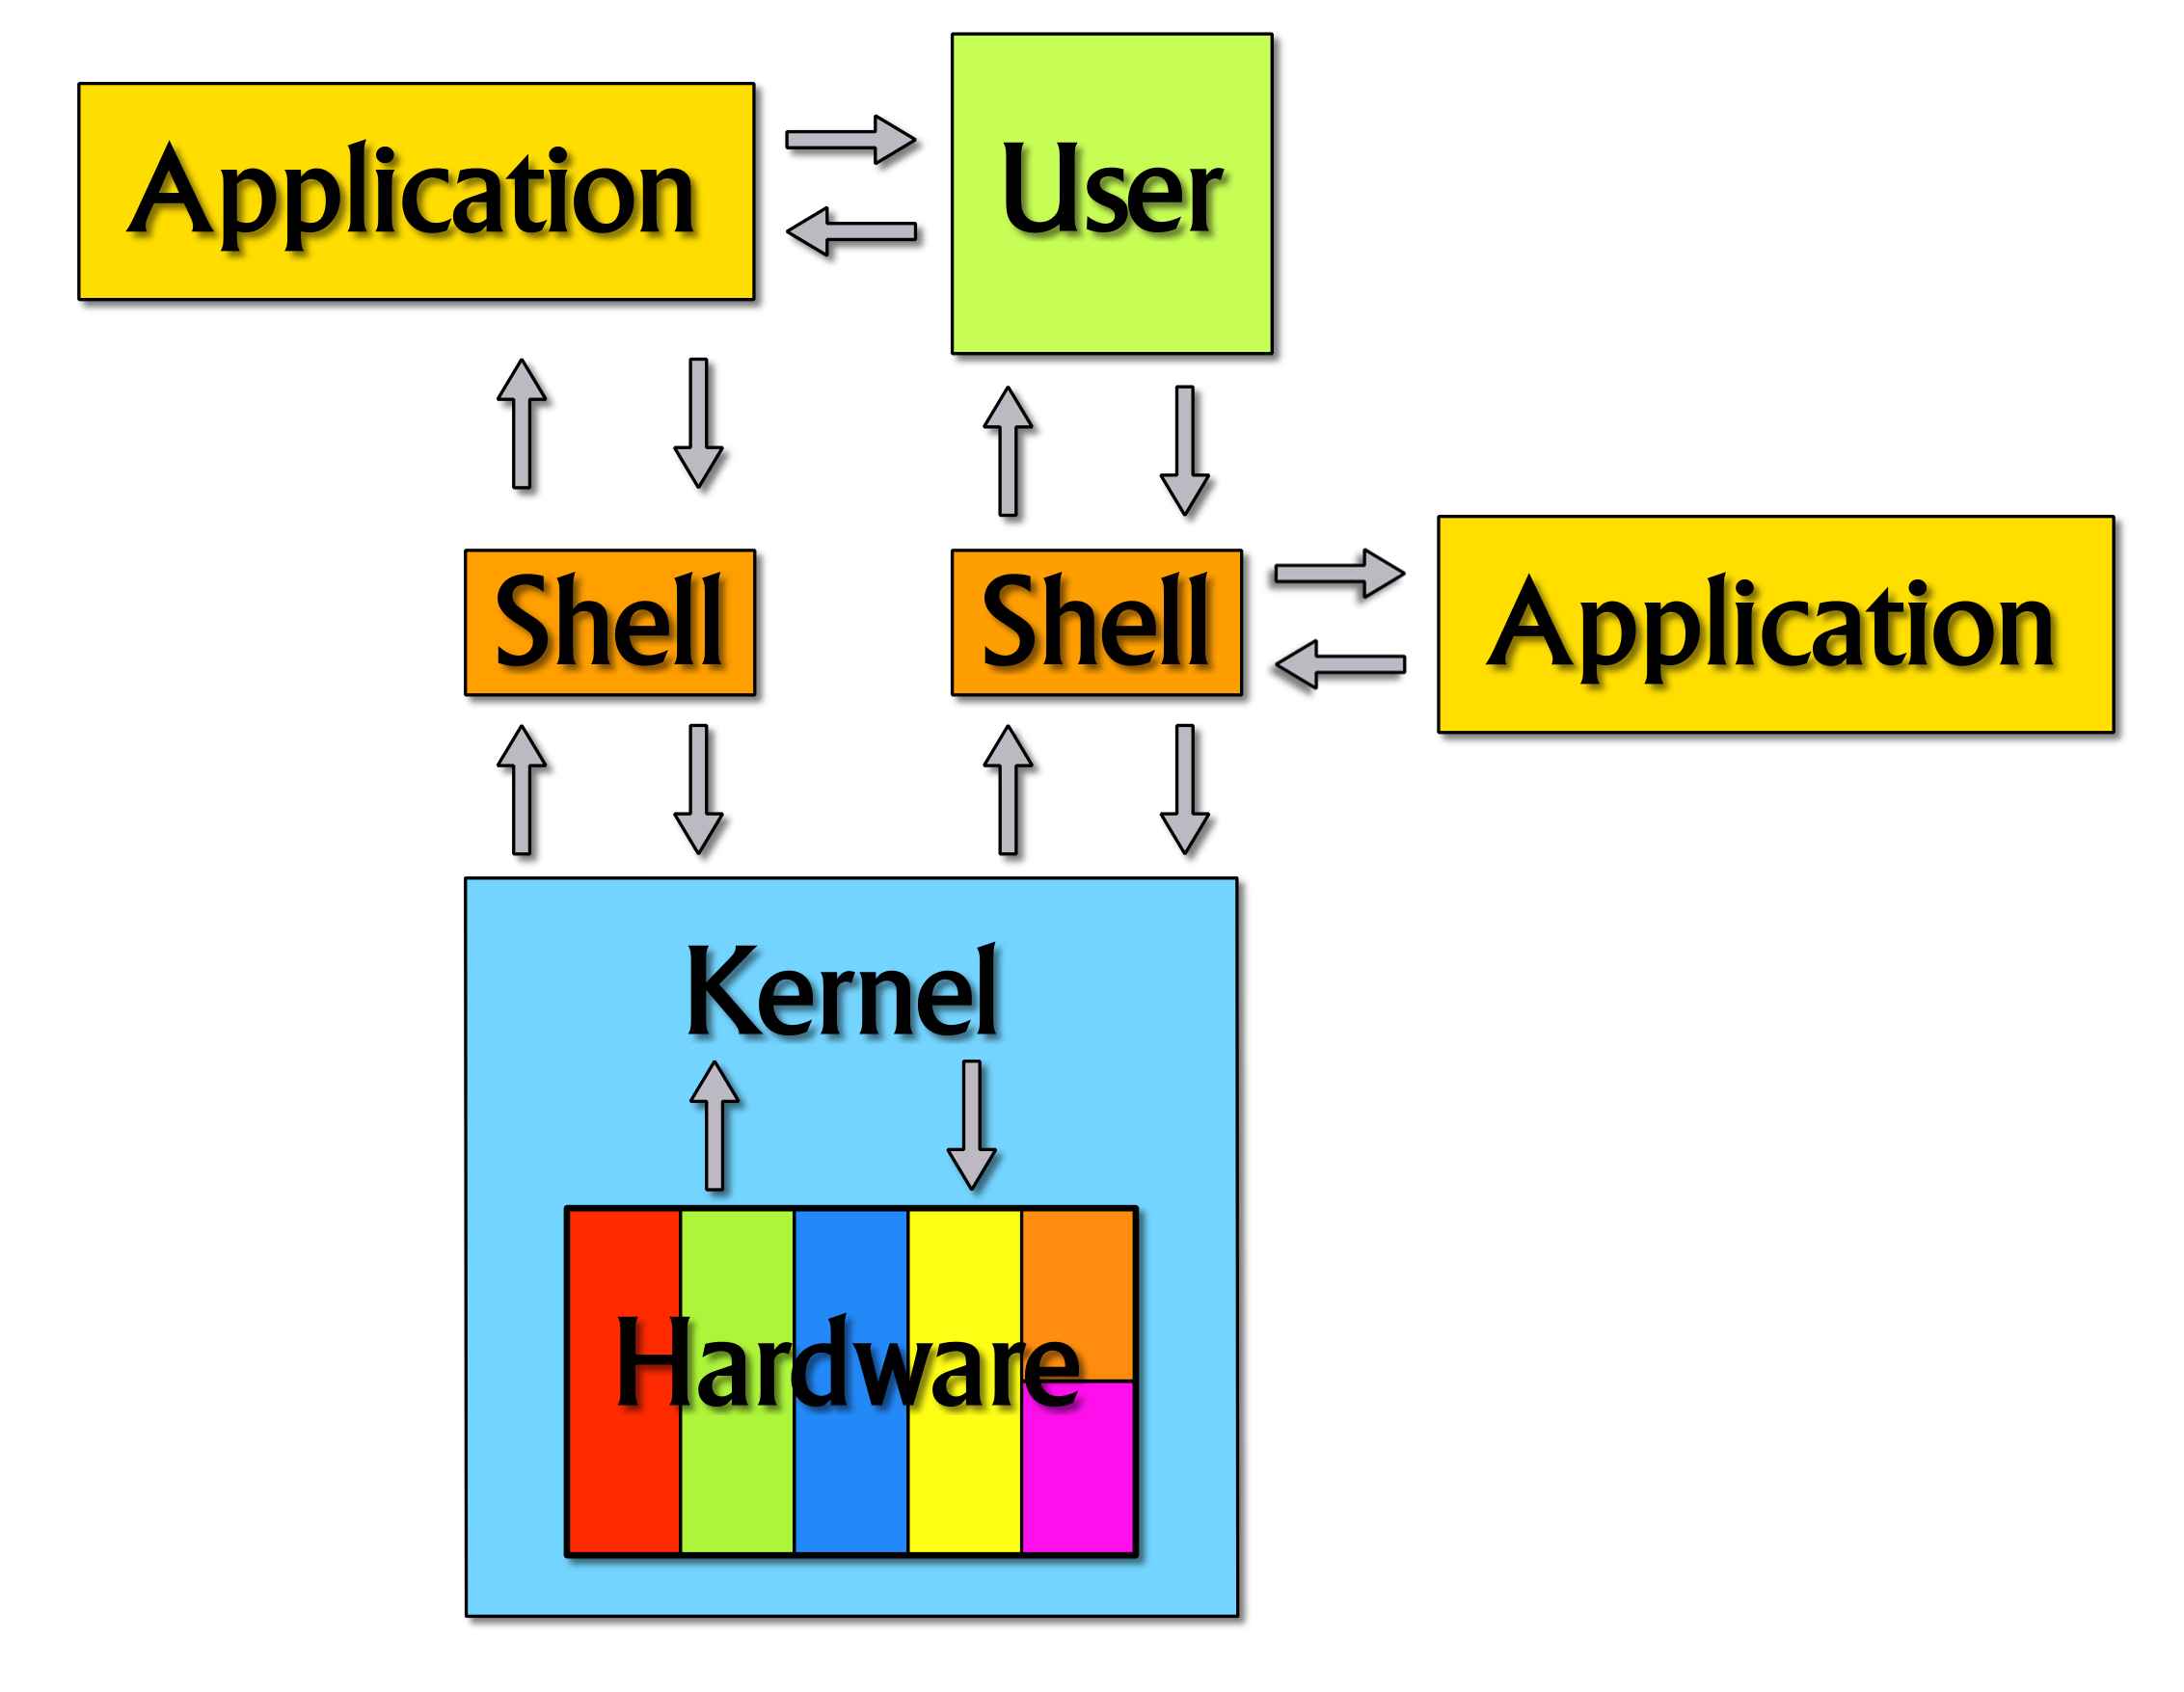
\includegraphics[scale=0.4]{Flow1.jpg}
    \captionof{figure}{Command Flow}
    \label{fig:user_flow}
\end{center}

Figure~\ref{fig:user_flow} is a diagram provided from opensuse at \href{https://en.opensuse.org/images/e/e2/Flow1.jpg}{https://en.opensuse.org/images/e/e2/Flow1.jpg} which goes deeper into how the user interacts with the system. You as the User will send commands to the Kernel using a Shell (in our case, Bash), where the Kernel then controls the Hardware. Think of the Kernel as a resource manager.

\section{Using Git with Windows} \label{Using Git with Windows}
Windows does not have a git client by default, so we will need to download software for that. This guide will utilize the popular \emph{git for windows}, or better known as Git Bash.
\subsection{Git Bash}
\subsubsection{Installation} \label{Win10-GitBashInstall}
On the Lab PC, enter the website \url{https://gitforwindows.org/} and click "Download". Once the download is finished, open the installer. All of the default options are good, sane options, so just keep clicking "Next" Until the installation is done.
\subsubsection{Using Git Bash}
When you are finished downloading Git Bash from Section \ref{Win10-GitBashInstall}, you can open up Git Bash by typing in "git bash" after pressing the windows key. Upon pressing enter, you will be greeted with a terminal that looks like the Figure~\ref{fig:win_06_Git_Bash}.

\begin{center}
    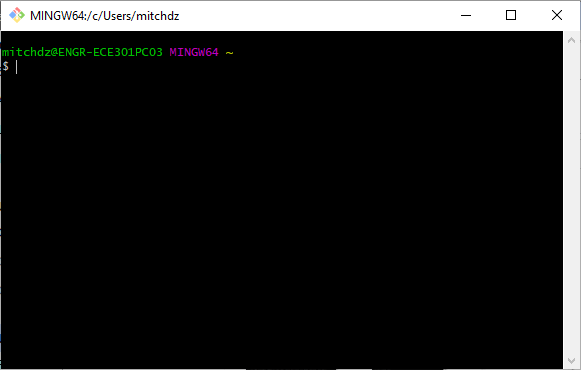
\includegraphics[scale=0.6]{win_06_Git_Bash.PNG}
    \captionof{figure}{Git Bash Default Screen}
    \label{fig:win_06_Git_Bash}
\end{center}

Now that you are in the terminal, you can use any commands that any usual bash terminal would have. You can enter the following command \textbf{(do not type the \$ at the start of the command, that is there by default)}:

\begin{lstlisting}
$ echo $PWD
\end{lstlisting}

\begin{center}
    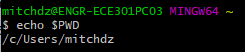
\includegraphics[width=3in]{win_07_echo_PWD.PNG}
    \captionof{figure}{Printing CWD in Git Bash}
    \label{fig:win_07_echo_PWD}
\end{center}

Figure~\ref{fig:win_07_echo_PWD} shows the result of running the above command. The result is "/c/Users/mitch". /c/ refers to the hard drive. "Users/mitch" refers to the path on that hard drive. The reason that you see the yellow tilde (that is the $\sim$ character), is that \textbf{$\sim$ is shorthand for "/c/Users/mitch"} (your username will show up instead of mitch).

You can change your directory into a folder where we can clone our repository. For this, we will be using the \textbf{cd} command. You can think of \textbf{cd} as standing for "Change Directory". Execute the following:

\begin{lstlisting}
$ cd Documents/
\end{lstlisting}

\begin{center}
    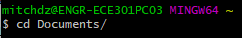
\includegraphics[width=3in]{win_08_cd_Doc.PNG}
    \captionof{figure}{Changing Directory to Documents}
    \label{fig:win_08_cd_Doc}
\end{center}

Figure~\ref{fig:win_08_cd_Doc} shows the results of changing our directory to Documents. You can now note that the yellow text says "$\sim$/Documents" which is actually referring to "/c/Users/mitch/Documents" in my case because the name for my User is mitch.

Let's create our own directory called 'git' in $\sim$Documents. This is where we will clone our git repository to be used for later.

\begin{lstlisting}
$ mkdir git
$ cd git
\end{lstlisting}

now you will be located in $\sim$/Documents/git. From here, let's clone a reference repository just to test everything. Execute the following command to clone an example repository with some Verilog code.

\begin{lstlisting}
$ git clone https://github.com/mitchdz/ExampleVerilogCode
\end{lstlisting}

now if you change directory into the new git folder you will see the code in the folder.

\begin{lstlisting}
$ cd ExampleVerilogCode
$ ls
\end{lstlisting}

















\begin{verbatim}
$ git commit -m 'init commit'

*** Please tell me who you are.

Run
eww
  git config --global user.email "you@example.com"
  git config --global user.name "Your Name"

to set your account's default identity.
Omit --global to set the identity only in this repository.

fatal: unable to auto-detect email address (got 'mitch@DESKTOP-AJ9NBNN.(none)')
\end{verbatim}

\clearpage
\section{Creating your own Github Repository}
There is a lot of software that utilizes git such as GitHub, SourceForge, Bitbucket and GitLab. For this guide we will utilize Github. To get some cool bonuses for being a student you can even register for the student pack at \href{https://education.github.com/pack}{https://education.github.com/pack}.





\section{Using Verilog Code from Github in Vivado}

\clearpage
\section{Advanced Git Commands}


\section{Advanced Bash Commands}

\end{document}